\documentclass[12pt]{article}
\usepackage[paper=a4paper,margin=2.7cm]{geometry}
\usepackage[utf8]{inputenc}
\usepackage{csquotes}
\usepackage{nameref}
\usepackage{graphicx}
\usepackage{amsmath}
\usepackage{textcomp}
\usepackage{eurosym}
\usepackage{float}
\usepackage{titlesec}
\usepackage{brufaceStyle}
\usepackage{setspace}
\onehalfspacing

\PassOptionsToPackage{hyphens}{url}\usepackage{hyperref}

\usepackage[sorting=none]{biblatex}
\addbibresource{references.bib}

\newcommand{\sectionbreak}{\clearpage}
\renewcommand{\contentsname}{Table of Contents}

\edef\restoreparindent{\parindent=\the\parindent\relax}
\usepackage{parskip}
\restoreparindent

\title{Master Thesis}
\subtitle{Analysis, via computer-based simulation, of the influence of a State's choices on efficiency, equality and happiness}
\author{Ricardo Gomes Rodrigues\\000443812}
\academicYear{2020 - 2021}
\promotor{Promoter: Prof. Hugues Bersini}
\masterAndMajor{Master of Computer Science}{Major in Artificial Intelligence}


\begin{document}

\maketitle
\newpage

\tableofcontents
\newpage


\section{Introduction}

An economic system is a very complex set of mechanisms and rules in order to produce, exchange and consume goods and services. Despite its complexity, this structure is a key part of our day-to-day life and we will try to understand different parameters of our system and their influences on key aspects such as efficiency, equality and happiness.

Unfortunately, such systems are virtually impossible to pin down analytically due to the many roles, rules and parameters: no set of mathematical formulas can model them properly. %TODO: Why more precisely? 
As stated by Leigh Tesfatsion, numerous algorithms have already tried to model social processes. We can cite a few of them such as genetic algorithms or reinforcement learning algorithms (Q-learning for instance). These algorithms have been developed with one purpose: optimality \cite{tesfatsion_bottom_up}.

In our case, we will use a computer-based simulation approach to study different types of economic systems. This approach will allow us to simulate a macro-structure (i.e. economic system) by the interactions of multiple autonomous micro-structures (i.e. agents) under a predefined set of rules. This approach falls into the area of Agent-based Computational Economics (ACE).

It goes without saying that such a simulation cannot model perfectly an economic system either, however it lets us see emerging patterns that can be studied and analysed to better understand how and why our systems work or do not work. The definition of a working system is not universal, but in our case we will settle for a definition based on the efficiency and the equality of our system as well as the happiness of its agents. 

This trade-off has previously been studied by multiple people, in particular in the paper wrote by Hugues Bersini and Nicolas van Zeebroeck titled \textquote{Why should an economy be competitive?} \cite{bersini}. It draws the conclusion that a \textquote{competitive market is efficiently superior to a random market, however, inequalities will be much more present}.

The aforementioned paper applied an ACE-based approach to \textquote{simulate the interactions of agents producing and trading goods within different market structures}. As previously stated, the agent-based method works well in case of a bottom-up approach: the agents, that can  produce, consume and exchange, will interact with one another. With large amounts of autonomous agents, we will be able to study emerging phenomena and see how the rules and parameters influence our economical system.

Our simulation will be made of different models all working together - similarly to a society. For this, we will introduce different concepts already mentioned in the previously referenced paper by Bersini and van Zeebroeck as well as new concepts that we will meticulously study later in section~\ref{section:motivation_objectives} based on the state-of-the-art research presented in section~\ref{section:state_of_the_art}. The models are described in the section~\ref{section:models} and an explanation of the implementation will be described in section~\ref{section:implementation}.

\section{Models}\label{section:models}

Agent-based computational economics (ACE) is part of a large class of agent-based modeling (ABM) which is a simulation modeling technique. This technique is used because we know that \textquote{even a simple agent-based model can exhibit complex behaviour patterns and provide valuable information about the dynamics of the real-world system that it emulates}.\cite{ABM}

ABM provides numerous benefits, as stated in \cite{ABM}. Amongst these, we can cite two key points that motivate this thesis: \textquote{ABM captures emergent phenomena and it provides a natural description of a system}. This is important because our goal is to have an empirical understanding of our system \cite{tesfatsion_handbook}, i.e., we want to understand why some systems work while others do not. And this will be done with in very intuitive way based on a natural description of ours models which will interact.
From a point of view of computer science, the object-oriented programming (OOP), seems to be the most suitable programming paradigm to implement our models and the system handling them. We will come back to that in later in the section~\ref{section:implementation} about implementation.

Nonetheless, we should also note some drawbacks of this approach; especially the issues revolving around social sciences such as irrational behaviour or subjective choices which are difficult to quantify and pin down mathematically \cite{ABM}. In order to simulate some irrational behaviour, we could introduce some non-deterministic behaviour where the agents would make a random choice from time to time. However, such a stochastic behaviour will be hard to calibrate. 
Another problem that may rise is the required computational power. Simulating such a complex system made of different models with many thousands agents is expensive. Therefore, we shall use tools that allow us to perform heavy computations as described in the implementation section~\ref{section:implementation}. 

ACE is a subclass of ABM where the focus is put on the simulation of economical systems where a \textquote{two-way feedback between microstructure and macrostructure has been recognised for a very long time}\cite{tesfatsion_complex_adaptive_systems}. Therefore we will use this methodology, which has proven itself, in order to study many questions present in the \nameref{section:motivation_objectives} section~\ref{section:motivation_objectives}.

We will now focus on the different models that make up our economical system: the products, the agents, the States, the market, and the World.

\subsection{Product}\label{section:product}
In the real world, we have two different types of products: the goods and the services. However, in this paper, we will not distinguish these two terms because the only thing that matters is that one producer and one consumer perform an exchange of a product in return of a certain amount of money. From now on, we will use the word \emph{product} to encompass these two words.

We should also note that by "exchange of product", we mean a sale-purchase relationship: after receiving the money, the producer does not have any right on the sold product anymore as opposed to a location or a license. We also assume that any product sold is directly consumed by the buyer and therefore will increase its happiness. The computation of the happiness will be described later in the section~\ref{section:actions} and will take into account the preferences (section~\ref{section:preferences}) of the agent.

\subsection{Agent}\label{section:agent}
We will focus on four key aspects of an agent: its assets, its actions, its skills and its preferences. The description here will be rather vague and is not definitive. It is supposed to give an overall outlook about what is present in the system and not how it works. The interactions between these models and their implementation will be described in the sections~\ref{section:implementation}. Each agent is unique. This will allow us to have an heterogeneous 'society' similarly to the one in which we live where each and every one of us has some skills and its own preferences.

\subsubsection{Assets}\label{section:assets}
Usually an agent owns multiple and different types of assets. In our case, we will focus on the financial and material ones. Indeed, an agent has a certain amount of money on its bank account. This amount is, needless to say, variable. 
However, each agent will start the simulation with a certain amount of money and afterwards, it will be up to it to spend it as it wishes (see section about preferences~\ref{section:preferences}) and also increase it by selling the products it produces (see section about skills~\ref{section:skills}). 
The amount of money an agent has will play a key part in the statistics that we will compute in order to study our study (for example to study the wealth distribution amongst agents). 

Our agent will also have material assets, namely the products it produces. It can only produce one type of products as described in section about skills~\ref{section:skills}. By producing a unit of a certain type of product, we increase the stock the agent has of that product. And, similarly, by selling a unit of a product, we decrease the stock if it was not empty. We can note that there is a lower bound (0 unit), but no upper bound (as many stocks as the agent wants).


\subsubsection{Actions}\label{section:actions}
An agent can be seen as a person who has both duties and rights. The agent \emph{can} produce, exchange (which encompasses the selling and buying actions) and consume products. These actions belong to the rights of the agent. Performing any of those actions will involve different components: a product, some money, a buyer (or consumer) and a seller (or producer) and the States to which our agents belong. 

However, we should also note that an agent has duties. Indeed, in our system we will introduce the concept of State in the section~\ref{section:state}. Because an agent belongs to a State, it \emph{has} to pay certain taxes. 
For instance, the well-known VAT (Value Added Tax) which has to be payed to the State each time an agent \emph{sells} a product. The rate the VAT will be State-dependent. Depending on a state, we may have different taxes that we will study to see how they influence our system. These multiple taxes will be explained in the section explaining a State, namely section~\ref{section:state}. All these taxes are examples of duties an agent has.

The actions involving a product are described as followed:

\paragraph{Produce}
Producing is the primary goal of an agent. However, an agent will not be able to produce at each time step (a tick as described in section~\ref{section:world}).
This will allow other agents (buyers, i.e., consumers) to have some time to buy our agent's products. Indeed, our agent should not produce all the time in order to avoid having too many stocks of unsold products because producing has a cost. This cost will be payed by the agent every time it produces one unit. 
An agent will not be able to produce indefinitely, we have an upper bound: the money available in its bank. We can note that the price of one unit of a product is withdrawn from the producer's bank, however, it does not go anywhere: we do not have a transaction, the money disappears from our system.

More details on \emph{how} the agent produces are available in the section regarding the skills (\ref{section:skills}) which will influence its production.

\paragraph{Sell}
After producing, it is obvious that the agent should sell its products to other agents: the buyer (or consumer). This represents a transaction involving two different agents in the system. However, not all transactions are allowed: stocks are empty, buyer has no money, the protagonists live in States tat have no connection (see section~\ref{section:state}).

\paragraph{Buy} 
An agent does not buy at every time step (tick), but when it does, it will analyse all its possibilities. It will choose one product it needs and try to find a seller. As stated before, not all sellers are equivalent because of their skills. However this is not the only criterion. Other criteria of seller selection are introduced in the section about its preferences. The goal of a consumer is to stick as close as possible to its preferences (section~\ref{section:preferences}) in order to maximise its happiness which is increased every time it buys/consumes a product. And, as for humans, some type of products may bring a bigger smile than others depending on multiple factors (product quality, product's origin or product's price for instance).

\paragraph{Consume}
When a buyer buys a product, we assume it consumes it directly. See previous section.

\subsubsection{Skills}\label{section:skills}
Since we are trying to mimic the reality as close as possible, an agent will have some skills regarding the production of each of the products available. Indeed, this means that it cannot be good at everything: humans need each other's talents.

Thus, each agent will have a list of abilities/skills associated to each of the available products. Because all agents should have equal chances, we will suppose that they all have the same total: an agent may perform will perform higher for some products, and lower in others. These will result in a mapping between the different products available in our simulation and the skill an agent has in the product: the skills will always be $\in [0, 1]$. Eventually, when adding up all its skills, each agent will have the same chances as others. We can do this by assuring that the sum of all its abilities equals to one.

$$\sum_{\text{product}} \text{product}_{\text{skill}} = 1$$

Higher skills in the production of one product bring, naturally, advantages to the agent. When it will sell its products, the agent will be able to build high-quality products and/or be able to sell them for a cheaper price. These two characteristics are determining factors whenever an agent buys a product as we will see in the next section.

\subsubsection{Preferences}\label{section:preferences}
We should now distinguish the preferences between two types of preferences: the preferences among different products and the preferences among different sellers of one product.

\paragraph{Product preferences} An agent will consume different type of products among the ones available in the simulation. Therefore, we will have, similarly to the skills, a mapping of preferences regarding each product. The higher a preference regarding a product, the higher the \emph{chances} are of picking this product when we buy one. One should be aware that these will be probabilities. The agent will not always pick the product with the highest preference value, however, this product will have more chances of getting picked.
We do this in order to let the consumer buy every product available in the simulation, and also because we see products as necessities. All of them are necessary, but some will be preferred to others as it happens in real life: we buy some necessary products that barely bring any happiness, and buy some other products which bring more joy to us.
As for the skills, the sum of all the preferences of each product have to be equal to one in order to force necessary products to have a chance at getting picked and each product preference is $\in [0,1]$.

$$\sum_{\text{product}} \text{product}_{\text{preference}} = 1$$

\paragraph{Seller preferences}
This kind of preferences will happen \emph{after} a product to buy has been chosen. Comparison between different sellers will happen here.
We may think that a rational agent would always pick the cheapest available option, however, as we can see in real life, this is not the case. Consumers have their own preferences, and it is not always the price! Indeed, we will introduce new definitions of rationality which used to be related to the price. These new preferences are based on the product's quality and its origin.

\begin{itemize}
    \item Because an agent has skills, it may produces some products better than others which result in a higher quality. Some consumers may prefer a more expensive product to a cheaper alternative because of its quality.
    \item Because our agents are assigned to States (see section~\ref{section:state}), an agent may prefer to consume local: it will buy a product from a seller belonging to the same State as it belongs to.
\end{itemize}

Happiness will be one of the key factors when we will analyse the simulation.

Finally, so far, we have supposed that our agents are rational. However, this is not always the case, and we will therefore allow some randomness in the consumer's choice so it does not always pick the same preference (price, quality or locality of the product) when comparing different alternatives (sellers).

\subsection{State}\label{section:state}
In this work, we introduce a new concept of 'State' which we will define as an entity containing multiple agents constituting a community operating on the same sets of rules.

\subsubsection{Rights and duties}
All of the agents in our simulation will be assigned to only one State: an many-to-one kind of relationship (multiple agents belong to one State). As stated previously, agents have some duties towards the State they belong to: taxes.

\paragraph{Duties}
Whenever an agent sells a product to another agent, it has to pay a certain amount to the State to which it belongs. This is an already existing concept: the Value Added Tax (VAT). This amount is computed as a percentage of the product's price. The VAT's value will be decided by the State. We will also try to introduce two other taxes:

\begin{itemize}
    \item the levy which is a contribution to the State. This levy will happen every time a certain number of ticks have been performed. The amount of this levy is fixed according to a certain percentage of the financial assets of an agent.
    \item a wealth tax which will not be payed by all agents, only the wealthiest. This tax is optional and not all States will impose it. It will be obligatory for agents whose financial assets are above a certain threshold.
\end{itemize}

\paragraph{Rights}
However, they also have some rights in regards to the State that are split in two categories: allowances and a universal basic income.

\begin{itemize}
    \item the amount of an allowance will depend greatly on the wealthiness of its receiver because its goals is to distribute wealth. 
    \item on the contrary, the universal basic income does not make any distinction between the agents. Every agent belonging to the same State will receive the same amount of fictional money.
\end{itemize}

Again, these two rights are subject to changes according to States. Each State may choose to use exclusively one of them, or it could also use none in case the State decides to limit wealth distribution.

\paragraph{Wealth distribution}
The taxes and allowances are introduced in order to limit the money difference between the richest and poorest agents and allow a better distribution of the wealth in the system. Because all these parameters are adjustable, different type of States will emerge.

Traditionally, States can, very roughly, be divided in three categories: pure socialism, pure capitalism or mixed. If a State decides to collect no taxes and offer absolutely no wealth distribution, we would label it as a pure capitalist economy. Conversely, if a State decides to opt for a planned economy (or pure socialism), every agent would work for the State it belongs to, and would not be able to increase its own financial assets.
However, most real markets today are not that extreme and fall into the mixed market category where some wealth distribution is present. This is a very simplified classification but it will suffice in our case to study and understand our simulation.

Wealth distribution will be one of the key factors when we will analyse the simulation.

\subsubsection{Connections}
The World we live in is very connected: States are very connected to one another and lots of exchanges take place across two different States. However, in our simulation, we will not connect them all in order to study the globalisation phenomenon. 

In our simulation, when two States are connected, we mean that a transaction may happen between a seller of one State A and a buyer from a State B. Therefore, if agents belong to two disconnected States, no exchange may happen between them. A State can have absolutely no connection to other States (very high level of protectionism), or be connected to multiple other States. This can be visualised as a graph as discussed in the implementation section (\ref{section:implementation}).

This allowed us to introduce the concept of "local preference" in the section regarding the consumer's preferences (\ref{section:preferences}). It will also allow us to introduce customs tax. Usually, when buying a product from another State, one has to pay some customs duty. These tariffs will vary from one State to another and are to be paid by the buyer.

An interesting form of connection that might happen will be clusters: groups of inter-connected States. Such clusters happen in real life such as the European Union where no custom taxes are collected when a transaction happens between a seller and a buyer from two different States. The same will apply in our simulation.

Figure~\ref{fig:connected_states} is an example of a graph of States where each vertex represents one State, green edges represent a connection of two States belonging to a cluster and grey edges represent a connection between two States. In this example, we can see that State can have no connection (vertex 0), or that a State belonging to a cluster can still have some external connections to other States which do not belong to the cluster (for example vertex 4 connected to vertices 8 and 12 with a grey edge instead of a green one).

\begin{figure}[H]
\centering
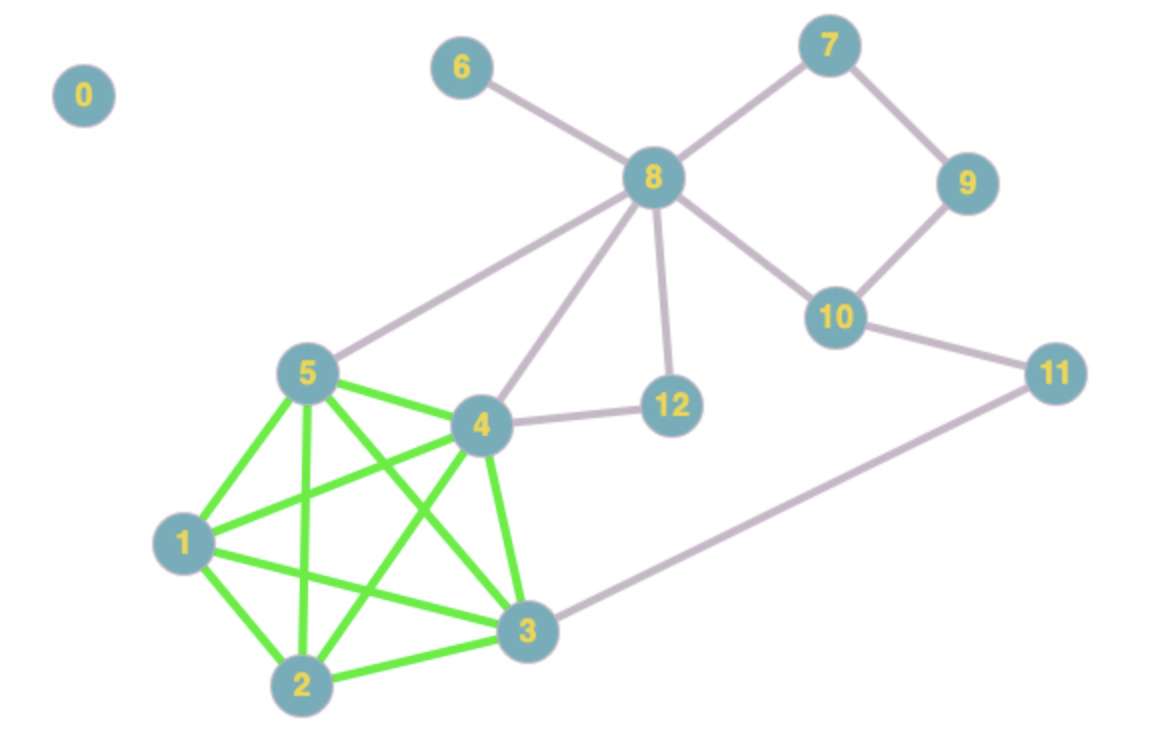
\includegraphics[width=0.7\textwidth]{img/connected_states.jpg}
\caption{Example of a graph of States}
\label{fig:connected_states}
\end{figure}

\subsection{Market}\label{section:market}
The market is an entity that will connect the agents. Its purpose is to allow interaction between agents of different States. It has no real functionality besides serving as a layer betwixt our agents and making sure both of them are allowed to exchange according to the rules that we have previously defined (sufficient stocks and money and connected States).

\subsection{World}\label{section:world}
After describing all our models, we eventually finish with the one that will encompass them all: the World. The purpose of this model will be to initialise all products, agents and States as well as let them be inter-connected through the Market.

The World will also handle the time step: a tick. Indeed, because computers are discrete machines, we have divide time into time steps (ticks). At each time step, our World will allow agents and States to perform actions such as producing, buying a product or collecting a tax.

However, as previously expressed, not all agents will perform an action at every tick. Only a certain percentage of the agents will do something: either produce, or buy, or do nothing (in case it has no money to either produce or buy, therefore it waits for someone to buy one of its products or for the State to give him an allowance). However, the action of selling may happen at anytime. This means that an consumer will be able to buy a product from a seller without waiting for him to also perform an action (otherwise, the system would be blocked very often).
This percentage value will be rather small due to the fact that a tick is something that will happen very often.

Finally, because our World contains all of the models we have defined (i.e. the products, the agents, the States and the Market), it will allow us to have an overview of all that is going on in our simulation. It will also be very useful in order to study the system and make some statistics.


\section{Motivation and objectives}\label{section:motivation_objectives}

The motivation of this work comes from my curiousness in understanding the World that surrounds us. Mixing social sciences with computer sciences is a very interesting way to give us some keys to better understand \emph{why} our economical systems is the way it is through a simulation. It would also be interesting to see what could be done to make the system better: either to make it more efficient or more equal.

\subsection{Objectives}

This work will have many objectives and a wide range of questions will be studied. Because our models will have many parameters, it will be very interesting to study their influence on the system. We have three main objectives which are an empirical understanding of the system, a theory generation of the system \cite{tesfatsion_handbook} and eventually an optimisation of the parameters.

In the former objective, the goal is to understand why some systems as we know them today have persisted. We will see which systems are viable and will not crash and see if it corresponds to the economic systems that we already know.

In the latter objective, the purpose it to understand the impact of parameters and see how the system changes under different initial conditions. The dynamics of the system might change heavily with some parameters, less so with others.

Finally, an interesting goal would be to optimise all the parameters that we have mentioned so far. Because the searching space of these numerous parameters is vast, we plan on using another algorithm to tweak these parameters in order to reach two different goals which are at the antithesis from one another: the amount of money present in the system and its distribution among the agents. However, this will be another topic to discuss in future work.

\subsection{Questions}

The main question that will be studied in this report is:

\vspace*{0.5cm}

\begin{center}
    How will the trade-off between efficiency and equality be affected by the parameters and choices we make when initialising our system?
\end{center}

\vspace*{0.5cm}

This question will depend on multiple factors that have already been studied in a real systems as we are going to see in the \nameref{section:state_of_the_art} section~\ref{section:state_of_the_art}. We will divide them into different categories representing the distinct models we have seen previously in the section~\ref{section:models}. 

\subsubsection{Products}

\begin{itemize}
    \item How will the number of products affect the EET (Efficiency-Equality Trade-off)?
\end{itemize}


\subsubsection{Agents}

\begin{itemize}
    \item How will the money that an agent receives at the beginning affect the EET? What if, instead of all agents starting with the same amount of money, we make some agents richer and poorer than others? This is useful to study the equality of opportunity.
    \item How will the agent's preferences affect the EET ? Will they make the agent poorer but happier? For example buying quality products might be more expensive but bring more joy.
    \item What would happen if some agents do not pay their taxes? Would do State crash if an important part of its agents do not pay them?
    \item Who are the happiest agents? Who are the richest ones?
    \item How important are the skills that an agent has? 
\end{itemize}

\subsubsection{States}

\begin{itemize}
    \item How will the VAT value affect the EET? Extreme cases might be useful to study to see clearer patterns such as what would happen if the State collects 100\% of VAT? What about 0\%?
    \item What about the customs tax?
    \item What about the levy rate ?
    \item How would a wealth tax affect the EET?
    \item Which redistribution system works the best? Decreasing allowances, Universal Basic Income (UBI) or none?
    \item Following the previous question, how important are the inequalities in such systems? What about the Gini coefficient? 
    \item How many connections does the State have? How does it affect the EET?
    \item How good (or bad) are the protectionism and the free trade policies?
    \item What is the importance of clusters? Do States that belong to a cluster perform better?
    \item How does the number of agents belonging to a State affect the EET?
    \item How happy are the agents belonging to a certain type of State?
\end{itemize}

\subsubsection{Market}
The market will have a global view and will focus on:

\begin{itemize}
    \item the money present in the system at each type step (efficiency)
    \item the distribution of the money in the system (equality).
\end{itemize}

and the relation between these.

Finally, we can see that most of the questions we will try to answer revolve around the State's choices and how it impacts its agents with regards to the efficiency, equality and happiness. This is the main goal of this research.

\section{State of the art}\label{section:state_of_the_art}
Besides the Agent-based Computational Economics (ACE) which has already presented, we will now focus on the state-of-the-art research related to the questions we have asked ourselves in the previous section.

Our goal will be to see if the state-of-the-art research presented hereunder does match the results that our simulation will yield. In future work, there will be lots of analysis and comparison between the two and see why this is (or this is not) the case.

\subsection{Taxes}

    The general consensus among the literature (\cite{burman2012taxes}, \cite{leigh2008redistributive} and \cite{taxes_inequalities}) is that a redistributive State limits the inequalities among its agents. And one way to do that is to levy different kind of taxes. A tax is defined as a compulsory financial charge paid by an agent (in our simplistic case) to the State in which it resides. 
    Nevertheless, in the rea life, the money collected by taxes is not only used to distribute wealth, but also to provide some common goods and services such as infrastructure (roads, street lamps, ...) or limited tuition fees.
    
    We will see different kind of taxes that might, or might not, be implemented by a State.

    \subsubsection{Value Added Tax (VAT)}
    
    The VAT is a rather modern tax which started to spread around the world in the late 1960s. Nowadays, the vast majority of the countries apply this tax also known under the name of Goods and Services Tax (GST) in some countries, however, not all of them do. It is not rare for a country to have multiple VAT rates for different kind of products (for instance one rate for necessary products and another for luxurious products).
    
    The VAT is a major source of income for the States that have implemented it. Indeed, the VAT accounts generally for more than 20\% of the total tax revenue in the countries of the Organisation for Economic Co-operation and Development (OECD) \cite{TheModernVAT}. Contrariwise, \textquote{the revenue-generating potential of the VAT is relative to a country’s administrative capacity. The VAT produces far less revenue, far less efficiently, in countries with weak administrative capacity.} \cite{OriginOfVAT}. According to the Table 1.5 of "The Modern VAT" \cite{TheModernVAT}, \textquote{countries that have implemented a VAT are relatively more developed}. 
    
    It interesting to note that the United States of America, the country whose GDP (Gross Domestic Product) is the highest, do not have a federal VAT. Instead, a sales and use tax is used in most USA states. In our case, there is no real difference between the VAT and the Sales tax because we only have one layer: the producer directly sells its product to the final consumer. Thus we will be using the VAT and Sales tax reciprocally. 
    However, it should be noted that, in the real world, the difference is quite important and we will very briefly describe it. In the case of VAT, each producer pays directly the VAT of the product it sold to the State, whereas in the Sales tax, only the final consumer will pay for it. Therefore, in the case of a Sales tax, the State has to "wait" for final good to be sold in order to receive the tax, whereas in the case of VAT, the State will receive the money gradually: only the 'added value' is taxed from one layer to another \cite{OriginOfVAT}.
    
    The standard VAT rate varies greatly between countries, from 0\% (in Hong Kong for instance) to 28\% in India (in the case of luxurious products). Albeit this rate may vary, a lot the majority of the countries in the OECD set it to be around 20\% \footnote{\url{https://www.oecd.org/tax/consumption-tax-trends-19990979.htm}}. Moreover, we can note that the European Union obliges its member states to have a standard VAT rate of \emph{at least} 15\% \footnote{\url{https://europa.eu/youreurope/business/taxation/vat/vat-rules-rates/index_en.htm}}.
    
    
    \subsubsection{Customs Tariffs}
    
    Whenever we import a product from another country, a certain amount of money has to be paid to the State in which the good is imported, this is known as tariff. It should be noted that the tariff rate usually varies from one product to another. This tax on customs is another tool that a State can use to levy money from its agents. Usually, this tax is a way to regulate and limit foreign imports in order to protect and stimulate domestic production.
    
    The rate of this tariff depends a lot from one country to another, and is a good indicator of the country's protectionism level. Indeed, it well known that the tariff's rate is a great tool to either boost or limit the trades between foreign countries. By setting a high rate, the imports will be greatly decreased and the local production will be favoured. Contrariwise, a low or null rate will encourage  free trade (thus leading to a globalised country) and a competitive market economy \cite{virmani2002towards}.
    
    In its very famous publication \textquote{Wealth of Nations}\footnote{\url{https://www.ibiblio.org/ml/libri/s/SmithA_WealthNations_p.pdf}} from 1776, when globalisation was very limited, Adam Smith advocates in favour of free trade which encourages economic growth according to him. Nowadays, the tariffs rate have generally drastically declined in comparison to the $19^{th}$ century as shown in Figure~\ref{fig:average_tariffs_history}.
    
    \begin{figure}[H]
        \centering
        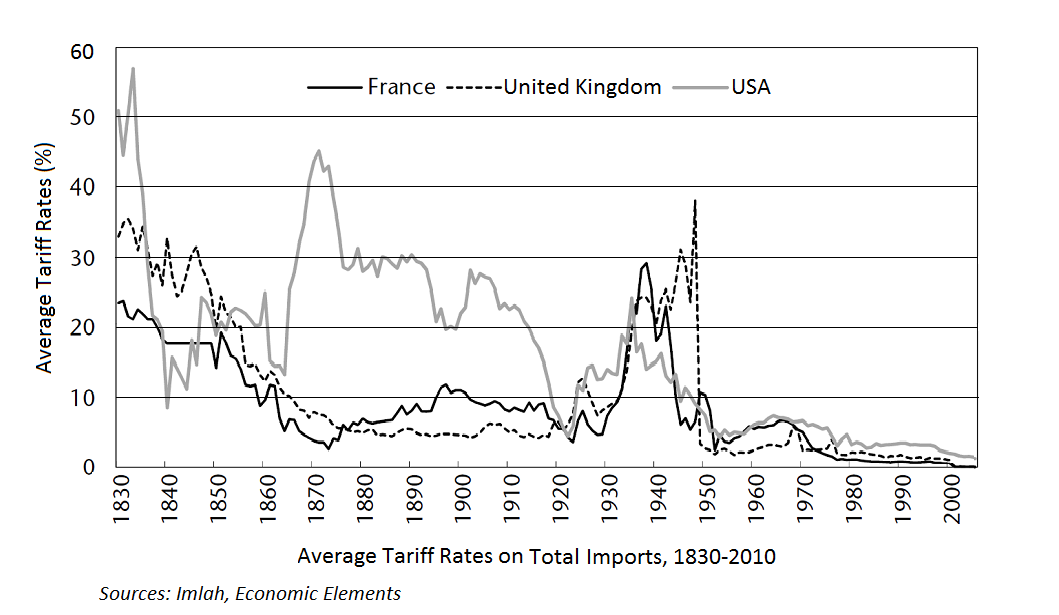
\includegraphics[width=0.7\textwidth]{img/avg_tariff_rates_US_FR_UK.png}
        \caption{Source: Wikipedia based on Albert Imlah's \textquote{Economic Elements}}
        \label{fig:average_tariffs_history}
    \end{figure}
    
    Albeit these tariffs have greatly decreased, many still exist in order to protect some at-risk domestic productions. However, nowadays, countries living in autarky (e.g. self-sufficient) are close to non-existent. Even North-Korea trades goods and services with countries such as Russia or China for instance.
    
    Today, the tariff rates all around the world vary from 0\% to roughly 20\%. A map summarising the average weighted tariff rate applied across all products is presented in Figure~\ref{fig:world_bank_tariffs}. This map is openly available on the World Bank's website\footnote{\url{https://data.worldbank.org/indicator/TM.TAX.MRCH.WM.AR.ZS?end=2018&start=2018&view=map}}.
    
    \begin{figure}[H]
        \centering
        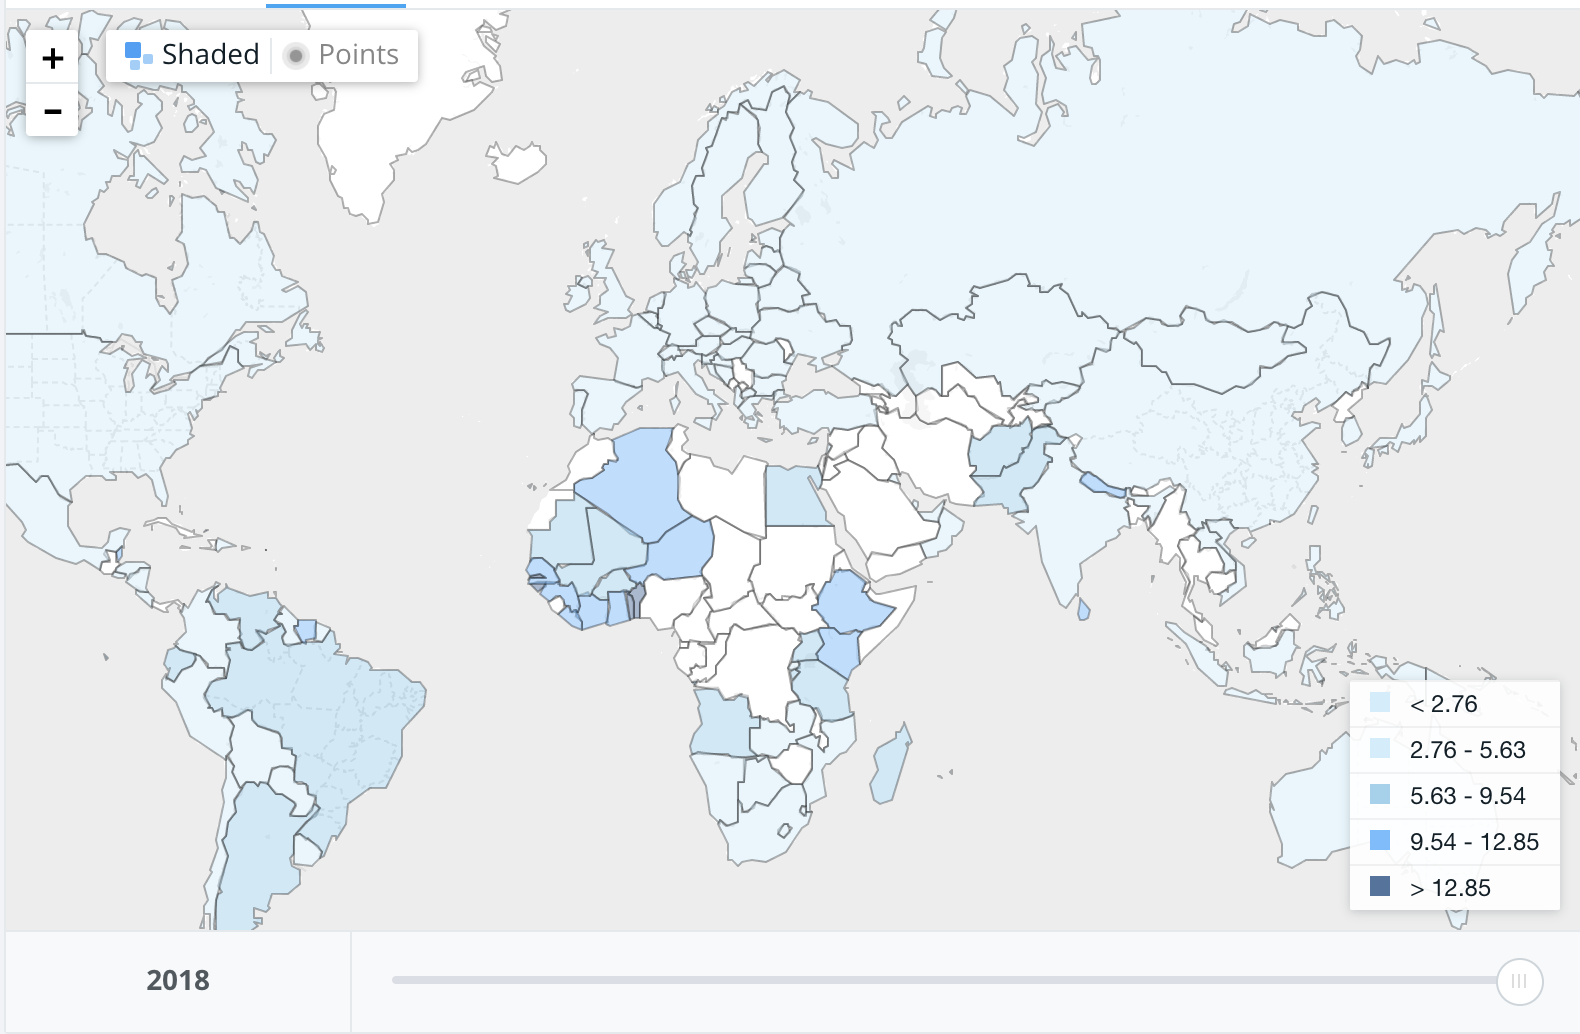
\includegraphics[width=0.7\textwidth]{img/world_bank_tariffs.jpg}
        \caption{Source: World Bank Data}
        \label{fig:world_bank_tariffs}
    \end{figure}
    
    Finally, we will note one very interesting case which is the tariffs rates of small countries, such as remote islands. "The Modern VAT" (\cite{TheModernVAT}) suggests that the advantages of a VAT will be greater than those of a tariff because of the large amount of imports.
    
    
    \subsubsection{Levy (contribution)}
    
    This levy tax can be seen as the income tax in the real world. Nevertheless, the levy tax in our model will be much simpler than the income tax which is a tax based on the income of a year, a time measure which does not exist in our timely discrete World made of ticks.
    
    This tax targets the income and profits earned by an agent, usually during a one-year period. This tax has been around for much longer than the VAT for instance as it appeared in the United Kingdom as early as 1799. In the great majority of the world, this tax is paid by an agent to the State in which it resides. It may be different in some countries (for example in the USA which taxes its citizens, even the non-residents ones), but this particularities go beyond our simulation which only knows the concept of residents.
    
    The income tax can usually be classified in one of the following categories:
    
    \begin{itemize}
        \item Proportional (or flat). In this case, the tax rate is constant across all income levels. The same marginal rate is applied no matter how much income is declared by an agent. Countries applying this kind of taxation include Romania, Russia, or Hungary. Some US states also collect a flat tax (in addition to the federal progressive tax).
        
        \item Progressive. In this case, the tax rate will increase as the income increases (by stages). This is the most used taxation category among the three. As shown by Giacomo Corneo \cite{progressive_taxation}, \textquote{tax progressivity might improve efficiency and the more so in egalitarian  economies}. Indeed, the poorer agents will usually pay a smaller tax rate whereas the richest agents will pay a higher a levy at a higher taxation rate. One should be careful, this is different from a wealth tax which is introduced in the next section~\ref{section:wealth_tax}.
        
        \item Regressive. Contrariwise to the progressive tax, this tax imposes a a greater burden on poorer agents. There are very few examples of such taxation systems.
    \end{itemize}
    
    As usual, the rates will greatly depend from one country to another. Some countries such as the United Arab Emirates do not levy any income tax whereas some countries can collect up to half of the income in taxes such Denmark or Belgium.
    
    \subsubsection{Wealth tax}\label{section:wealth_tax}
    
    The wealth tax is a taxation on the assets held by an agent. In our case, we will only take into account the financial assets, and more precisely the money an agent has in its "bank account".
    
    It is, once again, another tool that a State can use to increase its revenues. The idea of a wealth tax is as old as the Ancient Greek civilisation. Indeed, the symmoria \footnote{\url{https://en.wikipedia.org/wiki/Symmoria}} were a group of wealthy citizens that were grouped together with the purpose of collecting a higher tax: a wealth tax to put is simply.
    
    Nowadays, a wealth tax is present in several countries, but it not as generalised at other taxes such as the ones we have previously mentioned. This wealth tax is generally described as a certain percentage of the asset's which has to be paid to the State if the total amount of the assets exceeds a certain threshold. Multiple thresholds can be defined in order to have a progressive wealth tax. For example, taxing 2\% for assets worth more than \$50.000.000 and 6\% for assets worth more than \$1.000.000.000 (1 billion dollars). These are the numbers cited by US senator Elisabeth Warren \footnote{\url{https://www.cbsnews.com/news/elizabeth-warren-wealth-tax-who-would-pay-and-how-much/}}. However, a wealth tax can introduced starting much lower amounts. In Spain for example, the wealth tax starts gradually from 700.000\euro \footnote{\url{https://www.spanishpropertyinsight.com/tax-and-pensions/spanish-wealth-tax-patrimonio/}}.
    
    A huge drawback of the wealth tax is tax evasion and tax havens. Our imperfect simulation will not be able to take these into account unfortunately. According to Åsa Hansson, such a tax could dampen economic growth by reducing the level of investment. However the impact would be very limited.\cite{hansson2010wealth} Again, our imperfect system is not able to model investment and R\&D, therefore, the results in our simulation might be very different.


\subsection{Allowance and Universal Basic Income}

Because the State has collected money from different taxes, it will now have to redistribute it. In our simulation, there will not be any infrastructure or services that the agents can take advantage of such as public roads or free education. Therefore, all the money levied through taxes will go fully to the wealth distribution system which can be of two types in our system: either through allowances, or through the universal basic income (UBI). It is a exclusive choice, it is either one or the other, not both. So each fictional State will have to make a choice.

    \subsubsection{Allowance}
    
    An allowance is an amount of money given by a State to some of its citizens under certain conditions. The system handling this is called the social security whose role is to provide money to the less fortunate citizens. It insures that every citizen can afford, at least, the most basic needs such as food or shelter. Poorer people will usually receive more money than the wealthier who can already afford a better lifestyle.
    
    However, social security is not always a right in every country. Not all countries have implemented this safety net. According to the United Nations, the majority of the people across the world are not protected by a social security \footnote{\url{https://news.un.org/en/story/2010/11/359142-un-study-finds-most-people-worldwide-have-no-social-security}}. This social security is mostly available in developed countries whereas the percentage of people covered by such a system falls to around 5\% in sub-Saharan Africa.
    
    In our simulation, the social security will be a way of redistributing wealth in order to allow every agent to produce, consume and increase its happiness.
    
    \subsubsection{Universal Basic Income}
    
    Contrariwise to the allowances, in the universal basic income, we give the same amount of money regardless of the situation of each citizen. Everybody receives this amount of money periodically, no strings attached. The idea of a guaranteed income has been proposed throughout history (as early as the 16th century) and some countries have tried it but only for a limited period of time and only for a small sample of the population. Examples of countries that have tried UBI include Kenya, Finland and Macao but at relatively limited scale. 
    
    According to its advocates, the main reason why UBI will be necessary sooner or later is because of the rise of technologies which will replace humans and therefore making them jobless. Its ultimate goal would be to eradicate poverty by assuring everyone a decent amount of money for the most basic needs. And although it might seem Utopian and perhaps not perfect, Thomas Straubhaar, argues that it is worthwhile.\cite{straubhaar2017economics}
    
    However, its detractors critic the cost of such a system and its viability. Another argument is that, although some jobs will be lost, new ones will probably be created; the same way it was done during the industrial revolution. Finally, according to the critics, it is unfair because even the richest people would get this income. Robert Stephens rather suggests \textquote{to simplify and amend the current system, to make it fit  better  with the realities of the 21st century} \cite{stephens2019universal}.

    
\subsection{Economic clusters}
    As we have seen before, countries can impose tariffs on customs in order to discourage imports. However, what if countries had agreements between them in order to allow free trade (thus a null customs tariff) in-between a cluster? The most simple cluster would be made of two States freely importing and exporting from and to one another. This is known as a bilateral agreement. However, we can extrapolate this idea to more countries: a cluster made of a single market where no import tariffs would be levied by its member states.
    
    A very famous real-world example is the European Union (EU). The EU currently counts 27 member states exchanging in one single market with no tariffs on customs. The EU holds lots of advantages among these we can cite a few such as the freedom of movement or worker's protection across all member states, and the most important one being the large common market where goods and services can be exchanged at a cheaper price because of the lack of tariffs which also encourages investment.
    
    It also has some drawbacks such as the membership cost, the non-unique currency, and more bureaucracy. However, these will not be present in our simulation which does not model these aspects.
    
    We should also note that being in a cluster does not exclude a member state from having other bilateral agreements with other states.

\subsection{Efficiency/Equality trade-off}
    Finally, we will briefly discuss the broad question of the efficiency/equality trade-off and why it is a trade-off. Indeed, a trade-off means that improving one side will, generally, deteriorate the other side.
    
    This trade-off has actually been studied in previous works related to this one with the original work being the one of Bersini and van Zeebroeck: \textquote{Why should an economy be competitive ?}. This publication concludes that \textquote{a competitive market distributes welfare much less equally and is responsible for inequality amplifying effect} \cite{bersini}.
    
    In this work, another component has been added to the trade-off: the happiness. Indeed, an poorer agent may be happier than a wealthy one albeit it has less financial assets. No paper has approached this trade-off in such a way, and it will be very interesting to study this 3-component trade-off and how a State's choices influence it.


\section{Implementation}\label{section:implementation}

This section will give an outlook of how the code implementation will be structured. However, one should note that the structure in this section is temporary and might be subject to changes when the code will be developed during the Master Thesis.

\subsection{Code}
The code will be written from scratch and take inspiration from the code already written by Nicolas Bernier in Java for his master thesis titled \textquote{Comparison between a competitive and a redistributive market economy using computer simulation} \cite{nicolasbernier}.

It will be written in Java following the Object-Oriented paradigm which suits our simulation the best because of the different models that we have described earlier. Python3 is not excluded yet, however Java will be preferred because an agent-based simulation is a very power consuming task best suited for strongly typed and compiled languages such as Java (whose main paradigm is based on OOP additionally).

\subsection{GUI and visualisation}
A Graphical User Interface (GUI) will be implemented in order to let the user tweak all of the available parameters (number of products, agents, States, clusters, money from start, and so on). This will be a more user-friendly way than putting these parameters in a file. However this "advanced user" feature will also be available in the form of a configuration file (such as an XML or a JSON file) which would be more handy for advanced user who do not want to bother with a GUI.

Furthermore, another module will be developed to picture the system. This module will create different statistical graphs based on the simulation (for example the Gini coefficient measuring the wealth distribution in a system and the inequalities, the amount of money in the Market at each time step, etc.). It will allow us to study the different questions we have asked ourselves in the section regarding the objectives (\ref{section:motivation_objectives}) and also see the importance of the parameters and how they can change the result of a simulation.

\subsection{Class diagram}

Finally, a temporary class diagram is presented in order to better visualise the interactions between the different models. This class diagram is partially based on the one made by Hugues Bersini in its 2012 publication titled \textquote{UML for ABM} \cite{umbforabm} but with adjustments to fit the model we have previously described in section~\ref{section:models}. The class diagram is depicted in Figure~\ref{fig:class_diagram}.


    \begin{figure}[H]
        \centering
        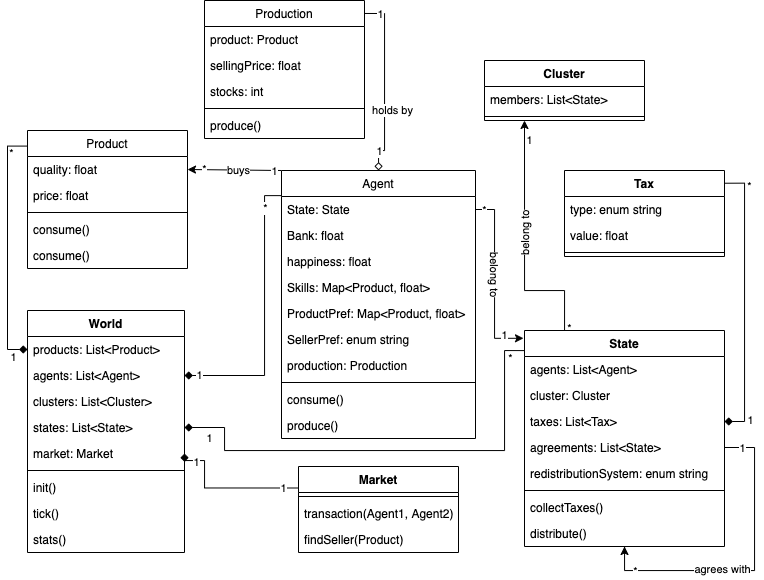
\includegraphics[width=1\textwidth]{img/class_diagram.png}
        \caption{Class diagram of the models}
        \label{fig:class_diagram}
    \end{figure}


\newpage

\section{References}
\printbibliography[heading=none]

\end{document}
